\section{Travaux de modélisations} 
\subsection{Modification du Modèle Conceptuelle de Donnée}

Pour permettre l'enregistrement des emprunts ainsi que des lieu d'emprunts il a fallu ajouter une table Location\_E (qui indique le lieu de location) ainsi qu'un table Bilioteque (qui indique le lieu d'emprunt) au MCD déjà existant dans Royal\_.
De même nous avons rajouté un boolean Enprunté\_A à la table Album afin d'indiquer si un livre est emprunté ou nous appartient.

\begin{wrapfigure}[1]{l}{13.5cm}
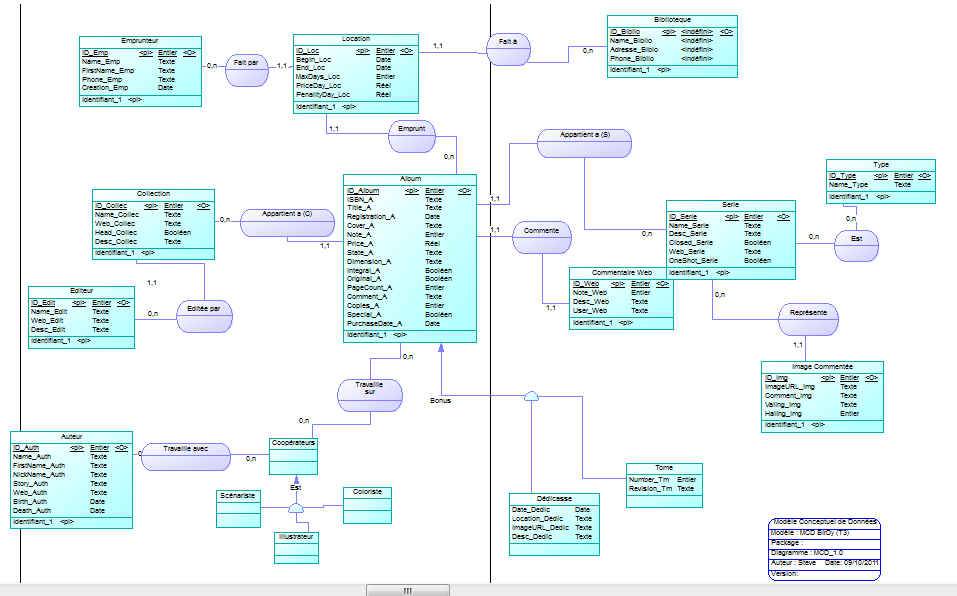
\includegraphics[width=13.5cm]{MCD_Royal_Modif.png}
\end{wrapfigure}
\clearpage{}

\subsection{Modéle Conceptuelle de Traitement}

Le MCT ci-dessous montre les différents traitement effectués dans Royal\_. C'est traitement seront présenté en fonction de leurs prioritées.
Nous pouvons observé tout d'abord la synchronisation d'ISBN (sur le client pc) présent dans la boite mail ainsi que la capture d'ISBN (sur le client android).
Ensuit nous pouvons voir que près la synchronisation si les albums sont loués une demande d'information sur l'emprut est executé (cette demande d'ajout d'information sur l'emprunt pet aussi etre effectué independament).
A coté nous pouvons voir le MCT concernant la verification des albums à rendre.
Enfin les deux derniers MCT traite de la synchronisation des Albums deja présents sur le client pc avec le client android.

\begin{wrapfigure}[1]{l}{14cm}
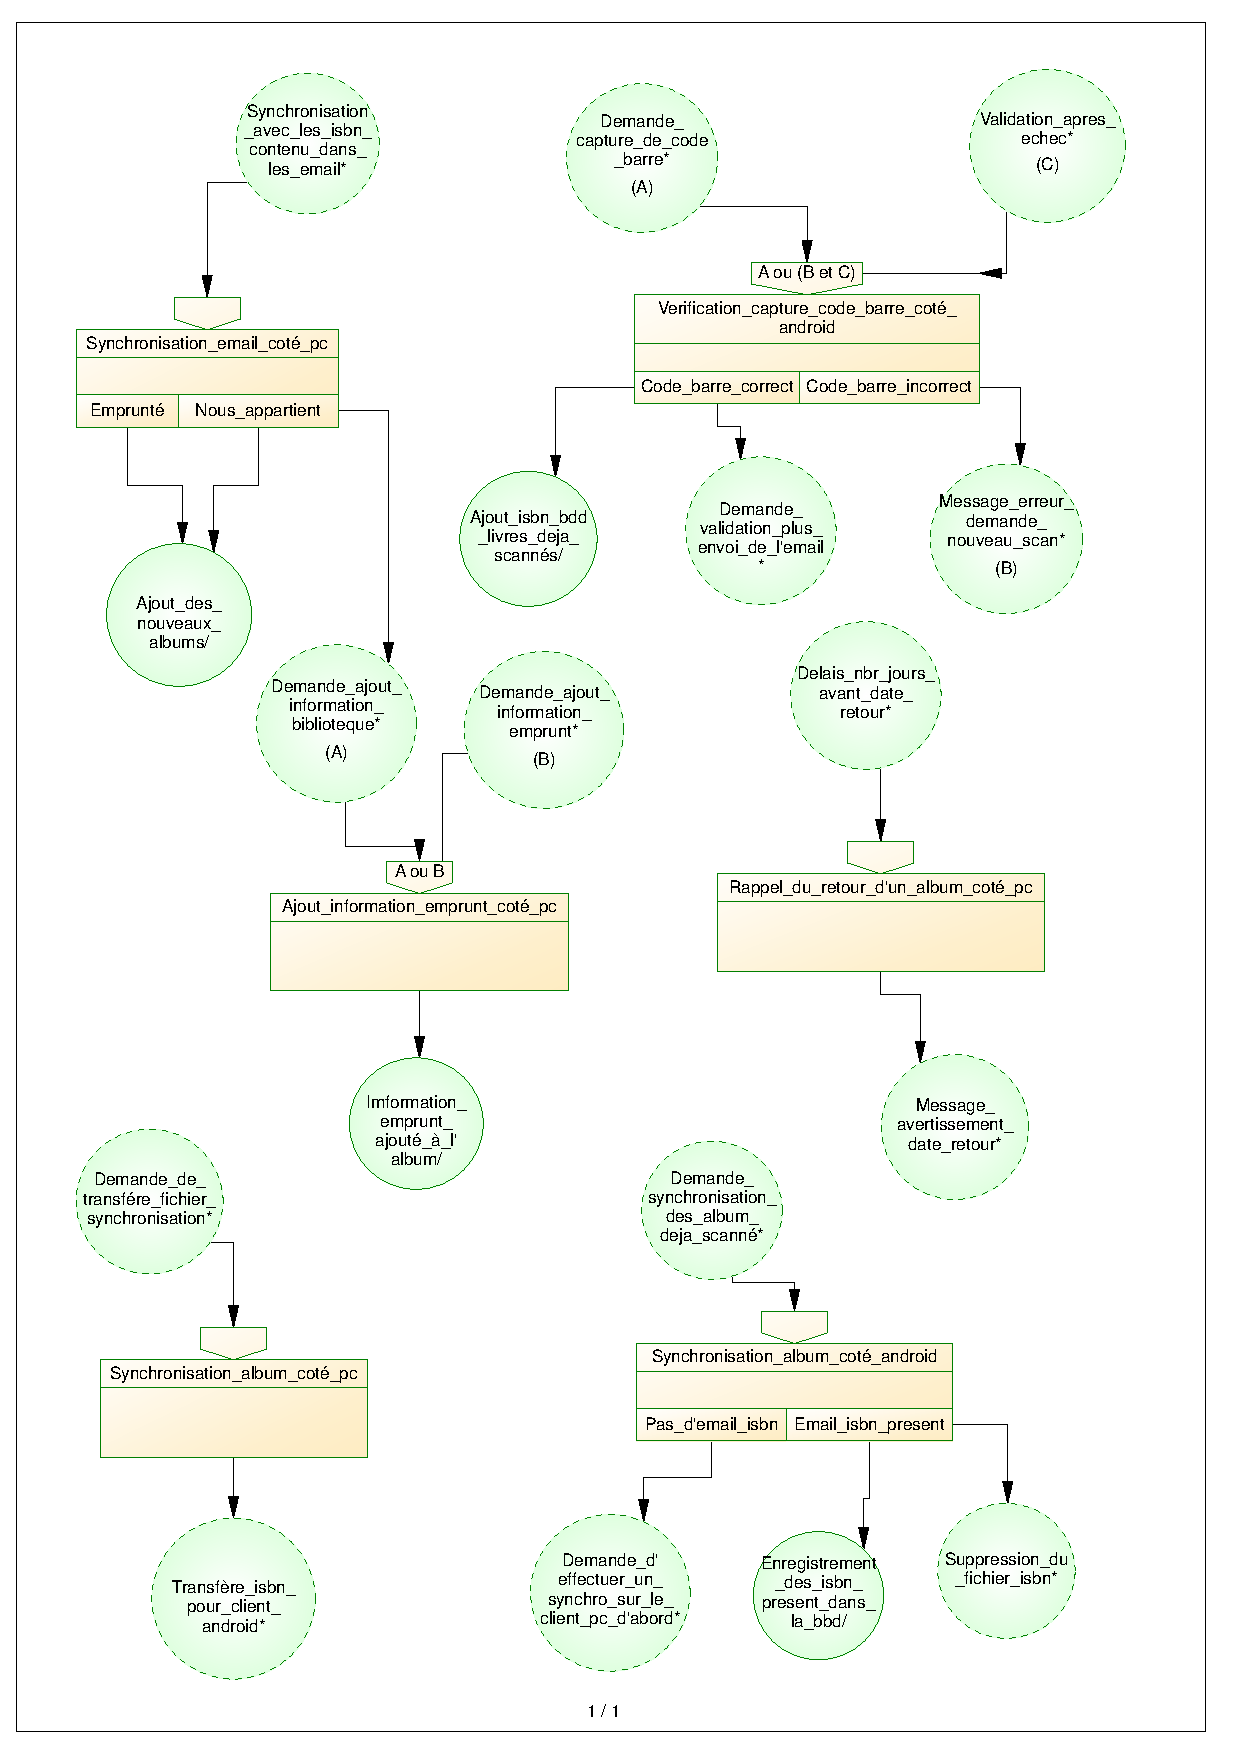
\includegraphics[width=14cm]{MCT_Royal.pdf}
\end{wrapfigure}
\clearpage{}

\subsection{Diagrammes d'activités}

\begin{figure}[h!]
\begin{center}
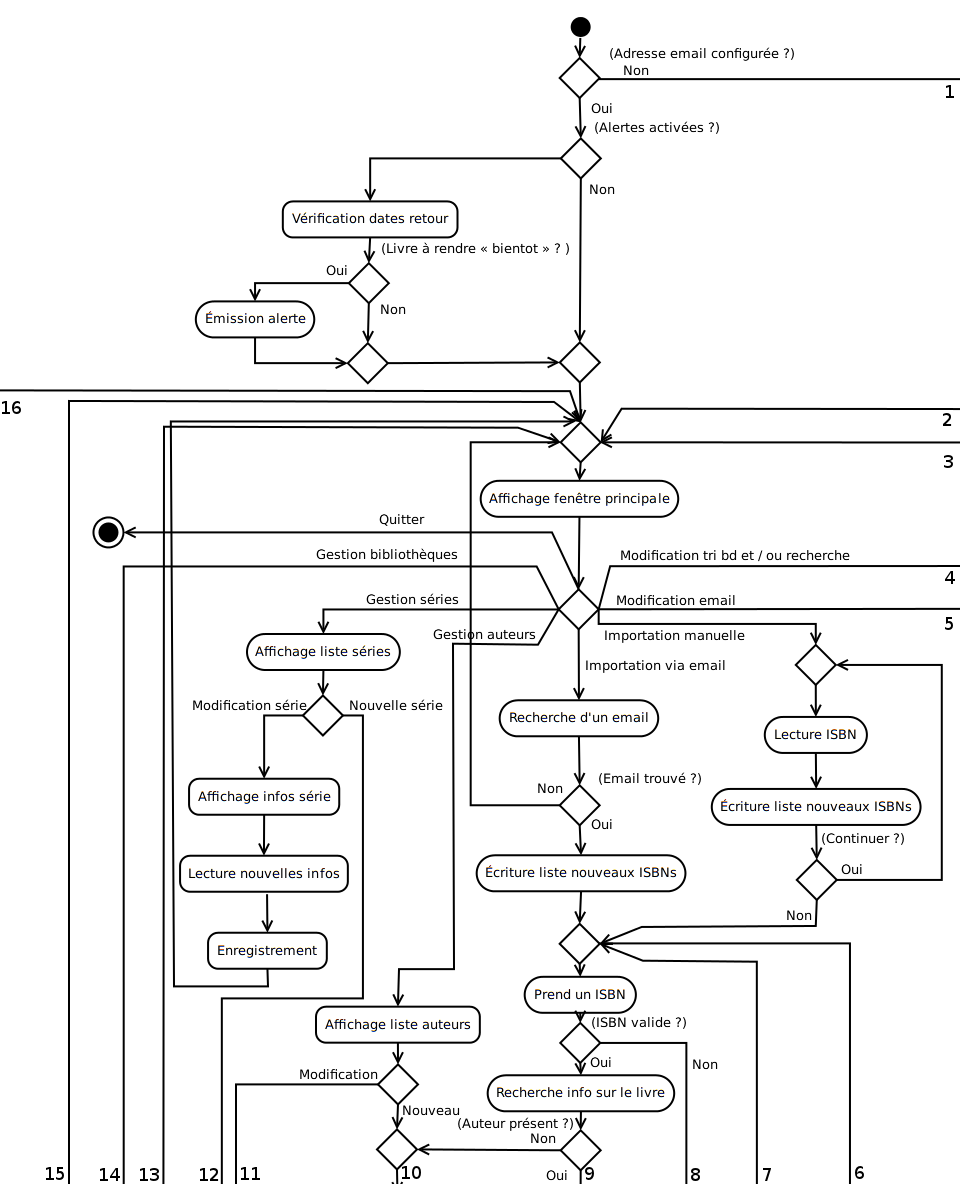
\includegraphics[width=16cm, height=19cm]{uml/appli_pc/p1.png}
\end{center}
\end{figure}
\newpage{}

\begin{figure}[h!]
\begin{center}
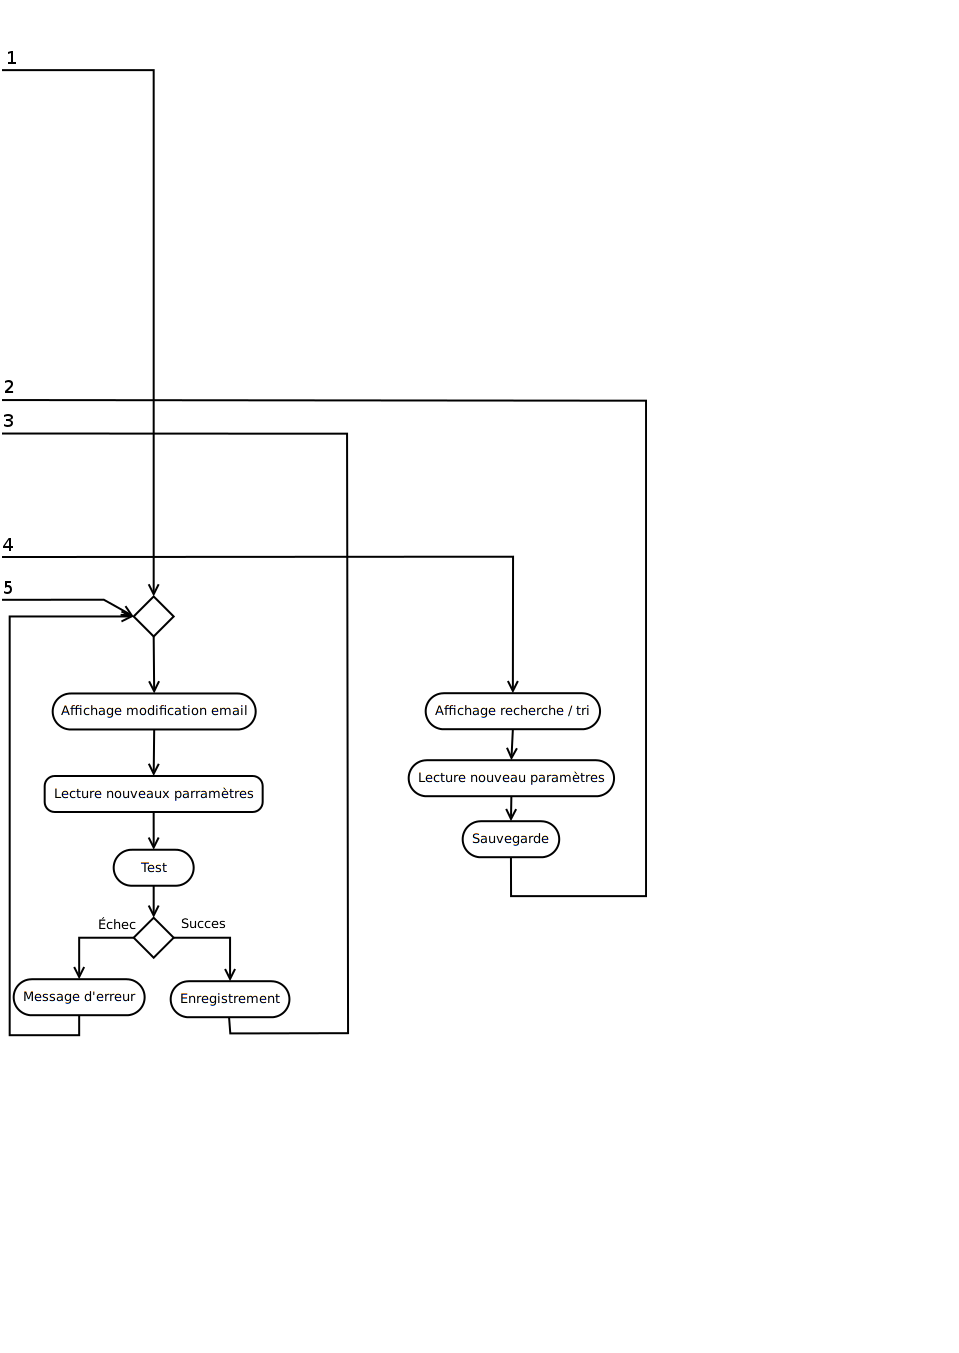
\includegraphics[width=16cm]{uml/appli_pc/p2.png}
\end{center}
\end{figure}
\newpage{}

\begin{figure}[h!]
\begin{center}
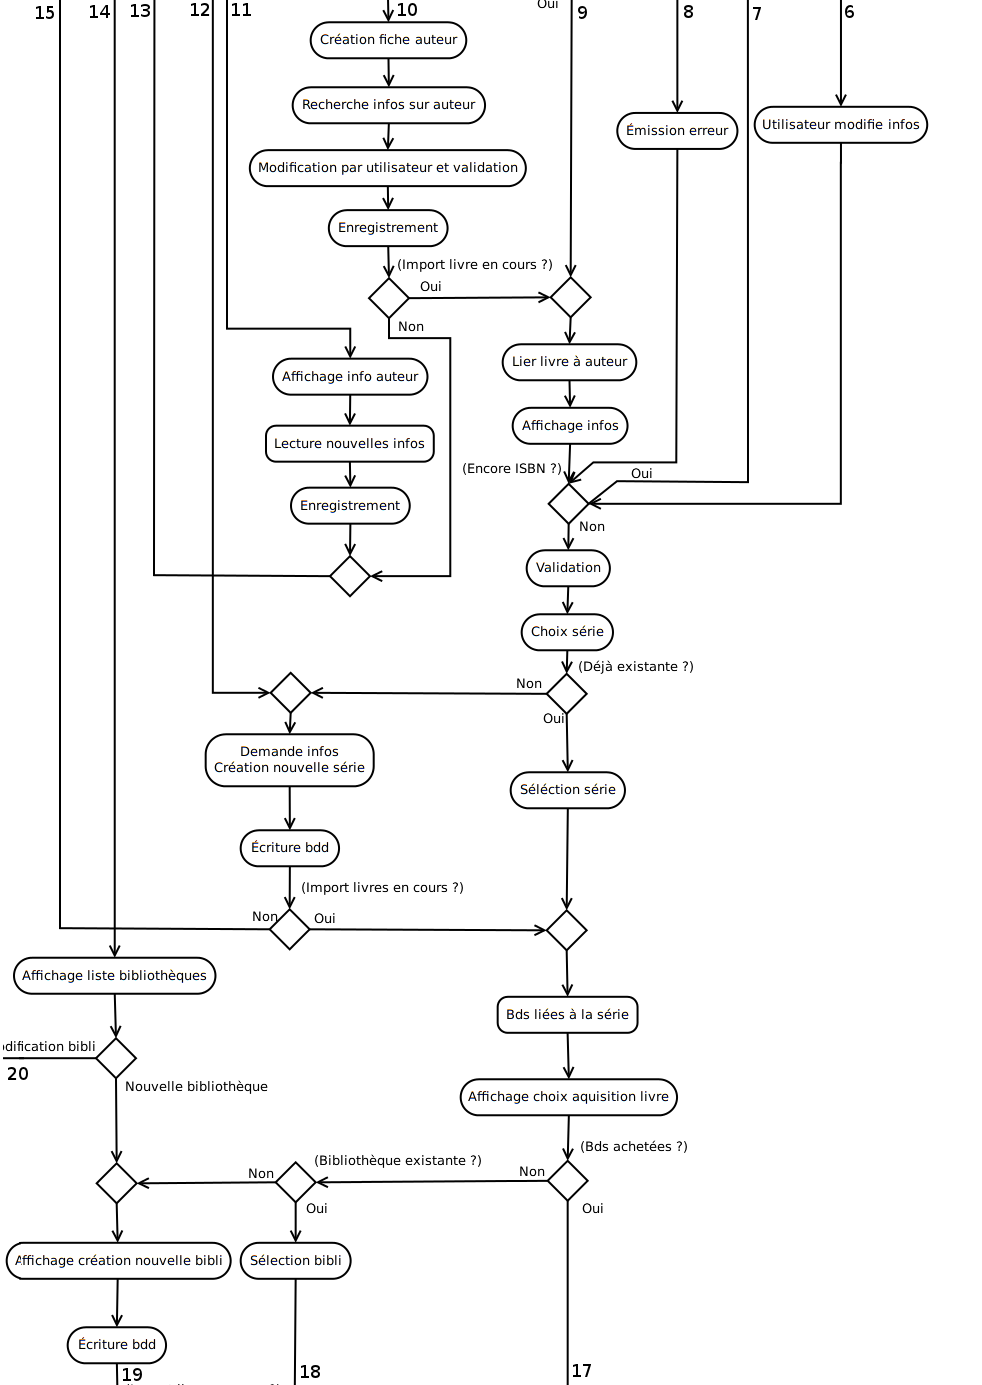
\includegraphics[width=16cm]{uml/appli_pc/p3.png}
\end{center}
\end{figure}
\newpage{}

\begin{figure}[t!]
\begin{center}
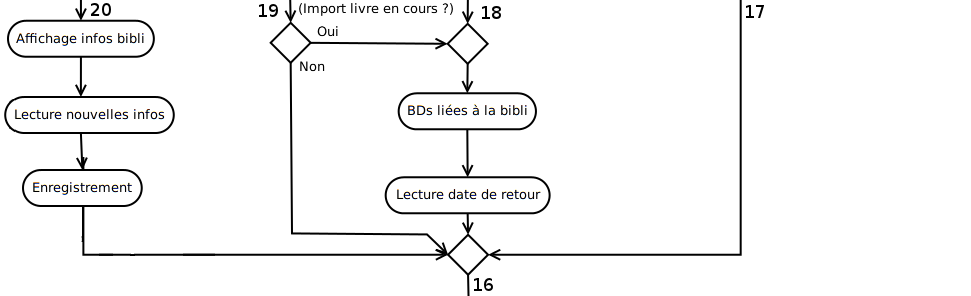
\includegraphics[width=16cm]{uml/appli_pc/p4.png}
\end{center}
\end{figure}

Une version plus lisible est disponible à l'adresse suivante : 
\emph{www.spyzone.fr/modules/images/pc\_application.png}

